\documentclass[11pt,a4paper,parskip=half]{scrartcl}
\usepackage{varioref}
\usepackage[utf8]{inputenc}
\usepackage[bookmarks=false,pdfborder={0 0 0}]{hyperref}
\usepackage{url}
\usepackage{listings}
\usepackage[svgnames]{xcolor}
\usepackage{graphicx}
\usepackage{amssymb,amsmath}
\usepackage{rotating}


% Standardformatierung für Quelltexte inkl. Sourcehighlighting usw.
\lstset{
  basicstyle =\color{black}\footnotesize,
  breaklines=true,
  backgroundcolor=\color{black!10},
  tabsize=2,
  breakatwhitespace=true
}

% Trademarks etc.
% http://www.danny4.de/archives/2006/02/15/latex-trademark-copyright-registered/
\def\TReg{\textsuperscript{\textregistered}}
\def\TCop{\textsuperscript{\textcopyright}}
\def\TTra{\textsuperscript{\texttrademark}}

% Take care of clubbing and widowing.
\clubpenalty = 10000
\widowpenalty = 10000
\displaywidowpenalty = 10000

\newcommand{\todo}[1]{{\color{red}\textbf{TODO:} #1}}

\newcommand{\programname}{{clj-net-pcap}}

%%%%%%%%%%%%%%%%%%%%%%%%%%%%%%%%%%%%%%%%%%%%%%%%%%%%%%%%%%%%%%%%%%%%%%%%%%%%%%%%%%%%%%%%%%%%
%%%%%%%%%%%%%%%%%%%%%%%%%%%%%%%%%%%%%%%%%%%%%%%%%%%%%%%%%%%%%%%%%%%%%%%%%%%%%%%%%%%%%%%%%%%%

\title{
\programname\\
Prototype
}
\author{
Ruediger Gad\\
}
\date{\today}


\begin{document}

\maketitle

\tableofcontents

\listoffigures

\section{Description}
\programname{} is a wrapper/adapter/facade (Whatever you wanna call it.) for using jNetPcap \cite{jnetpcap} with Clojure \cite{clojure}.

\section{Requirements}
Clojure 1.3

Java 1.6

Operating Systems: Linux and Windows (both x86 and x86\_64) 
See also below on which configurations \programname{} could be successfully run and on which not.

For Linux \texttt{libpcap}\cite{libpcap} version 1.0.0 or later must be installed.
For Windows \texttt{winpcap}\cite{winpcap} version 4 or later must be installed.

For building the distributable Jar file etc. and running the unit tests Leiningen \cite{leiningen} is recommended.

\programname{} has been successfully tested on: 
Linux (Fedora 16)  x86\_64 libpcap 1.1.1

Note that Windows seems not to provide an \texttt{any} device.
Also note that there seems to be some issue with respect to the libpcap based filtering mechanism on Windows.
Here no filter should be set (via the \texttt{-f ""} option) for first tests.

\section{Running}
\subsection{\programname{}}
\label{sec:running}
Generally, \programname{} must be run as a user with the permissions required to list all network interfaces, to set a network interface into promiscuous mode, and to inject packtes into a network interface.
Ususally, this means \programname{} needs to be run as root or Administrator respectively.
For a guide on how to capture packets as non-root user in Linux see: \url{http://packetlife.net/blog/2010/mar/19/sniffing-wireshark-non-root-user/}.

\subsection{Unit Tests}
Most of the unit tests need to have full access to the network interface in order to sniff data.
Hence, the tests need to be run as a user with the according permissions, e.\,g., as root / Administrator.
For running the unit tests simply execute \texttt{lein test} from projects base directory.

\section{Architecture}
The main work is done in two threads (see Figure \vref{fig:simple_data_flow}).
The ``Sniffer Thread'' is responsible for sniffing data from the network interface.
This sniffed data is stored in a queue.

From this queue the ``Forwarder Thread'' reads the data and processes/forwards it further.
At this point essentially anything could be done with the data:
e.\,g., print to \text{stdout}, or write to a file.

The functiones that are used as packet handler and forwarder can be set via command line options.
For more information see how \programname{} is started (see \vref{sec:running}).

\begin{sidewaysfigure} 
  \centering
  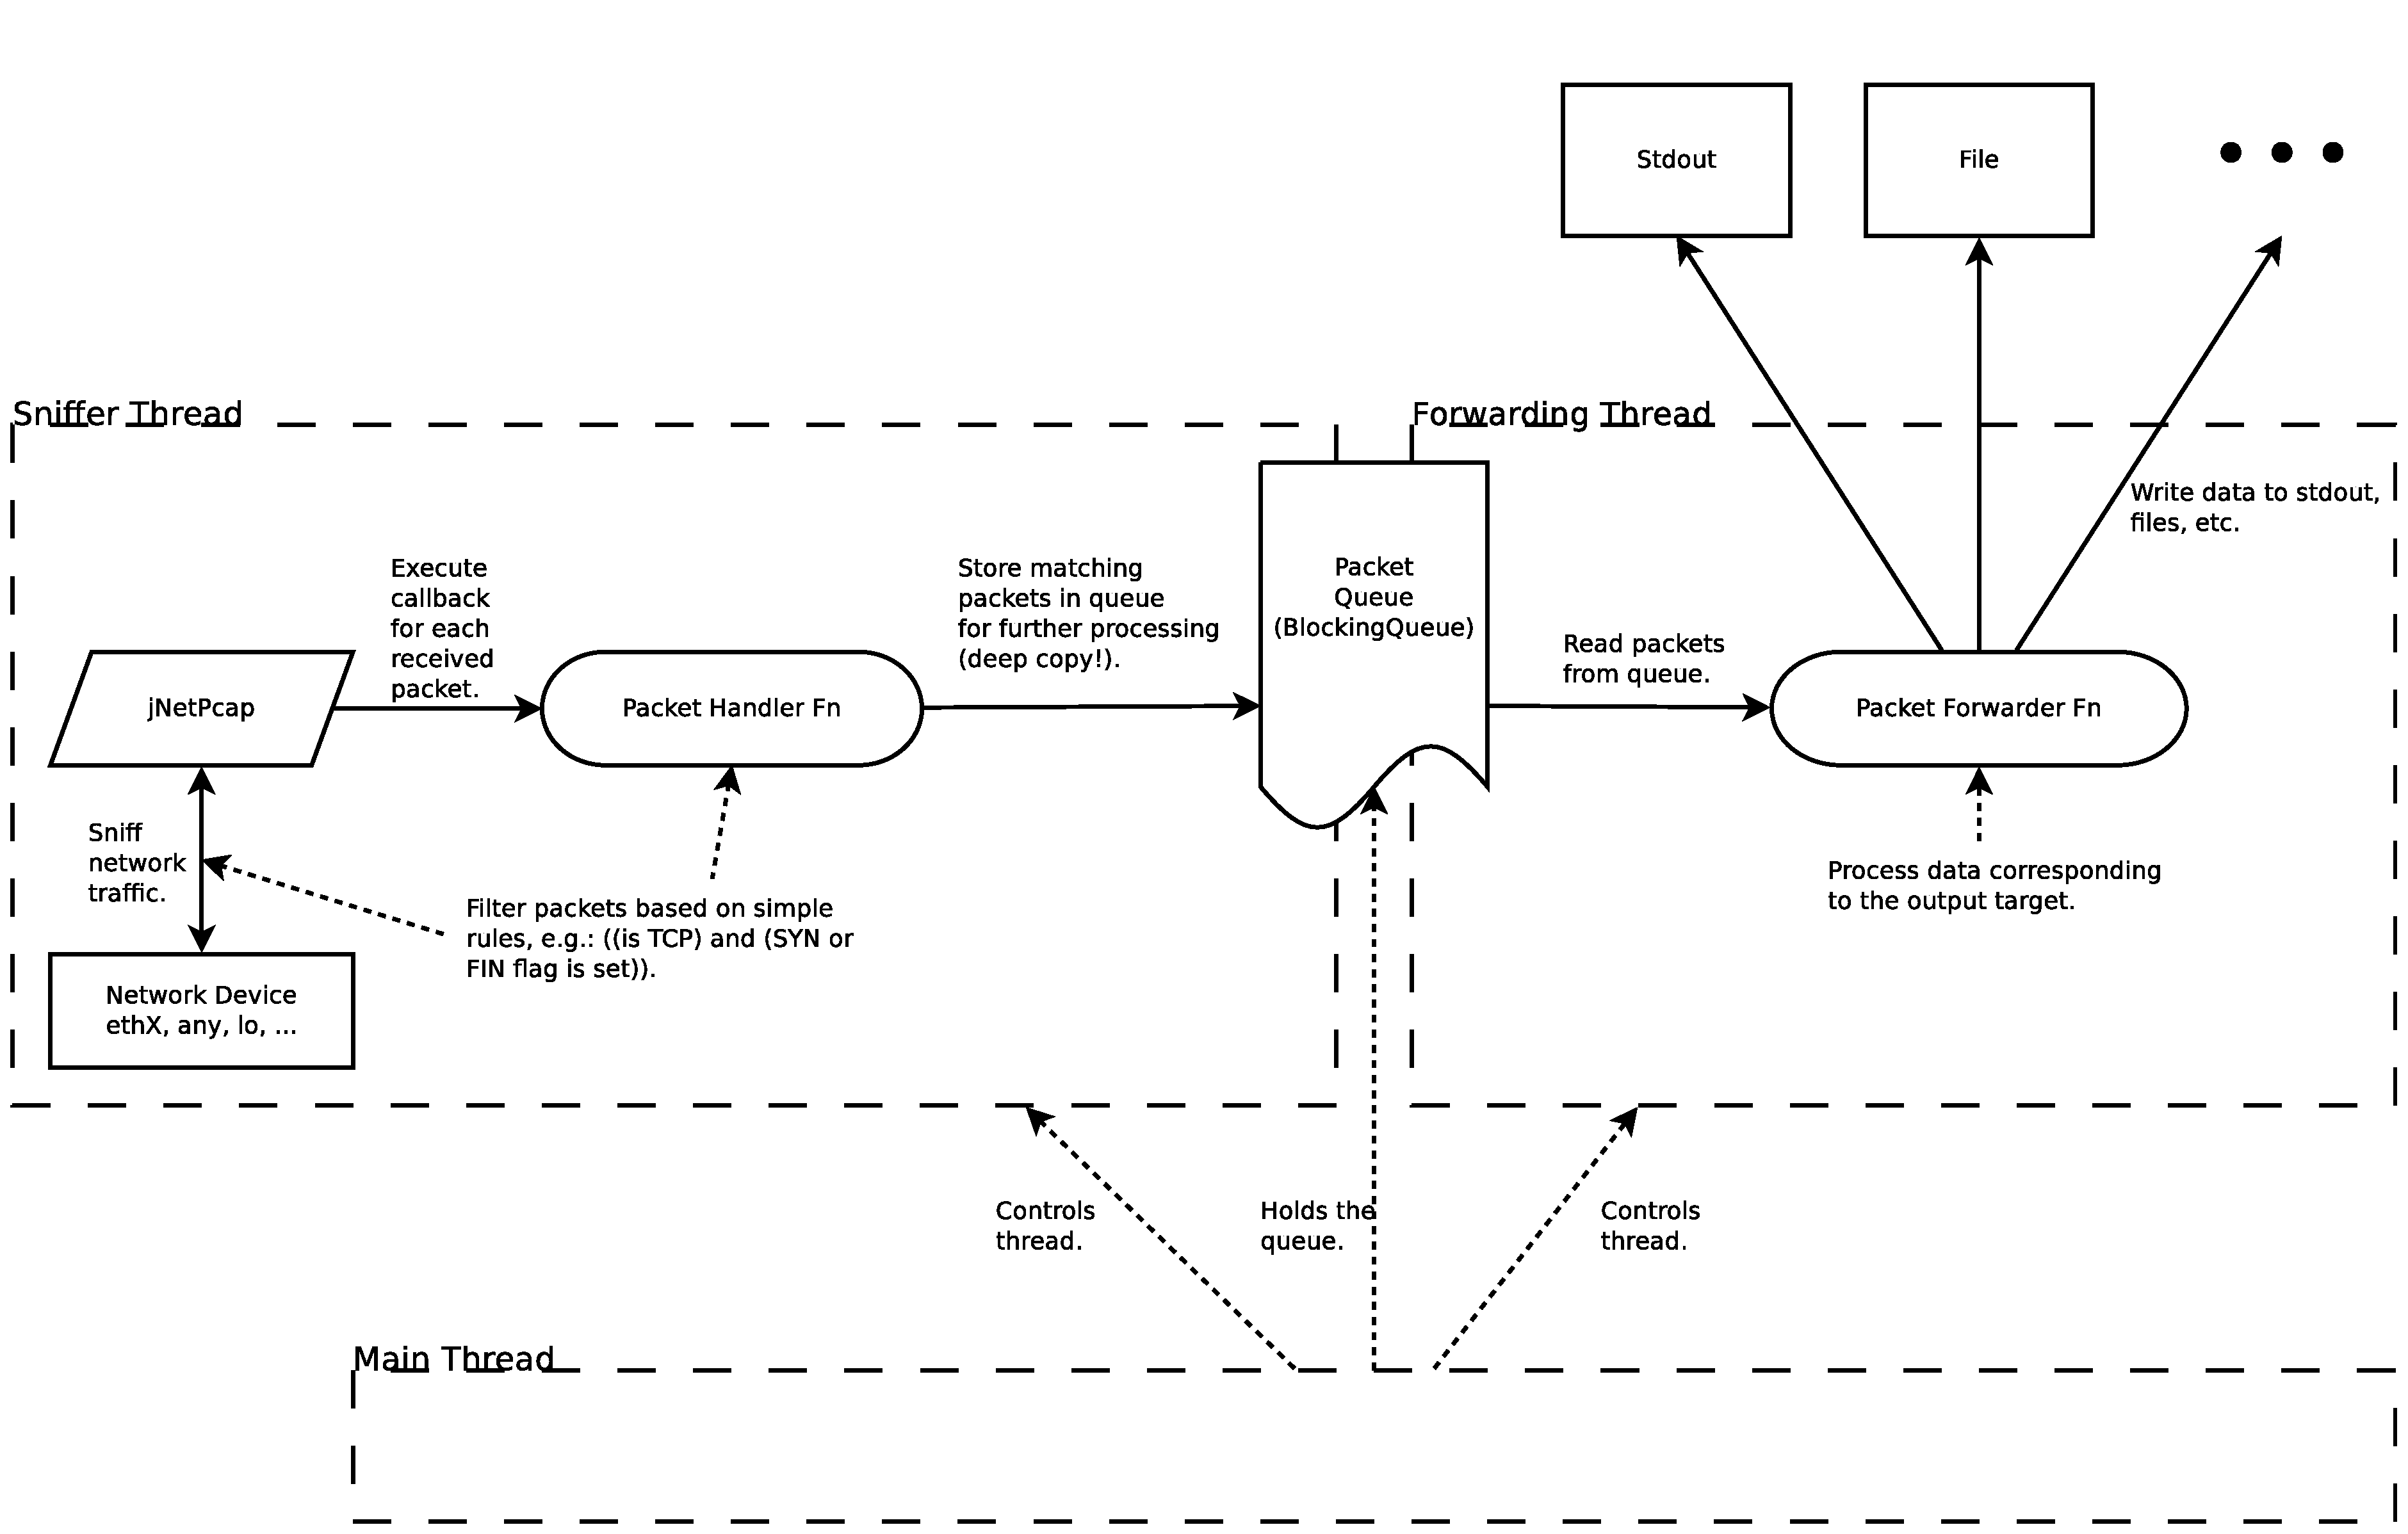
\includegraphics[width=\textwidth]{diagrams/simple_data_flow}
  \caption{Simple Data Flow Diagram}
  \label{fig:simple_data_flow}
\end{sidewaysfigure}

\subsection{Filtering the Input Data}
The input data can be filtered at two points:
first, native libpcap filters can be used to filter the packets prior to sniffing (default).
In this case only matching packets will be sniffed.
Second, the already sniffed packets could be filtered in the Clojure packet handler code.

\subsection{Forwarding the Data}

\bibliography{bibliography}{}
\bibliographystyle{plain}

\end{document}
